\documentclass[a4paper, 11pt]{article}
\usepackage{comment} % enables the use of multi-line comments (\ifx \fi) 
\usepackage{lipsum} %This package just generates Lorem Ipsum filler text. 
\usepackage{fullpage} % changes the margin
\usepackage[a4paper, total={7in, 10in}]{geometry}
\usepackage[fleqn]{amsmath}
\usepackage{amssymb,amsthm}  % assumes amsmath package installed
\newtheorem{theorem}{Theorem}
\newtheorem{corollary}{Corollary}
\usepackage{graphicx}
\usepackage{caption}
\captionsetup[figure]{name={图}}
\captionsetup[table]{name={表}}
% \usepackage[pdftex]{graphicx}
\usepackage{tikz}
\usetikzlibrary{arrows}
\usepackage{verbatim}
\usepackage[numbered]{mcode}
\usepackage{float}
\usepackage{tikz}
    \usetikzlibrary{shapes,arrows}
    \usetikzlibrary{arrows,calc,positioning}

    \tikzset{
        block/.style = {draw, rectangle,
            minimum height=1cm,
            minimum width=1.5cm},
        input/.style = {coordinate,node distance=1cm},
        output/.style = {coordinate,node distance=4cm},
        arrow/.style={draw, -latex,node distance=2cm},
        pinstyle/.style = {pin edge={latex-, black,node distance=2cm}},
        sum/.style = {draw, circle, node distance=1cm},
    }
\usepackage{xcolor}
\usepackage{mdframed}
\usepackage[shortlabels]{enumitem}
\usepackage{indentfirst}
\usepackage{hyperref}
\usepackage{CJKutf8}
    
\renewcommand{\thesubsection}{\thesection.\alph{subsection}}

\newenvironment{problem}[2][Q]
    { \begin{mdframed}[backgroundcolor=gray!20] \textbf{#1 #2} \\}
    {  \end{mdframed}}

% Define solution environment
\newenvironment{solution}
    {\textit{Solution:}}
    {}

\renewcommand{\qed}{\quad\qedsymbol}
%%%%%%%%%%%%%%%%%%%%%%%%%%%%%%%%%%%%%%%%%%%%%%%%%%%%%%%%%%%%%%%%%%%%%%%%%%%%%%%%%%%%%%%%%%%%%%%%%%%%%%%%%%%%%%%%%%%%%%%%%%%%%%%%%%%%%%%%
\begin{document}
\begin{CJK}{UTF8}{gbsn}
%Header-Make sure you update this information!!!!
\noindent
%%%%%%%%%%%%%%%%%%%%%%%%%%%%%%%%%%%%%%%%%%%%%%%%%%%%%%%%%%%%%%%%%%%%%%%%%%%%%%%%%%%%%%%%%%%%%%%%%%%%%%%%%%%%%%%%%%%%%%%%%%%%%%%%%%%%%%%%
\large\textbf{课程: 人工智能} \hfill \textbf{作业 1}   \\
北航软件学院 \\
\normalsize 学期: 2024，春季\hfill 提交截止时间:  2024年4月11日, 11：59 PM \\
\noindent\rule{7in}{2.8pt}
\textbf{提醒注意:}
\begin{itemize}
\item 本次作业发布于2024年3月22日，截止于2024年4月11日。
\item 作业一分为三部分：问答题、实训题、以及实训题报告
\begin{itemize}
    \item 问答题答案可以手写并扫描，或者用latex（或word）手打，最终以QA.pdf文件命名。
    \item 实训题按照项目共享链接内要求和基础代码进行作答。
    \item 报告部分同样可以手写或者手打，以Report.pdf文件命名。
    \item 作业提交格式：$<student ID>$\_$<name>$\_A1.zip。比如ZY1921102\_田嘉怡\_A1.zip
    \item 提交的zip文件要求（仅）包括：
    \begin{itemize}
        \item 实训题文件：包括 spam.py 和 y\_private\_pred.npy文件
        \item 问答题答案：QA.pdf
        \item 报告：Report.pdf
    \end{itemize}
    
\end{itemize}
\item 作业压缩包需要在spoc平台上提交。
\item 每迟交1天（不满1天按1天计算），本次作业扣除10\%分数。
\item 不按作业要求和格式提交，视情况扣分。不得抄袭。
\end{itemize}

\noindent\rule{7in}{1pt}
\textbf{第一部分：问答题（共4分，每题1分）}
% %%%%%%%%%%%%%%%%%%%%%%%%%%%%%%%%%%%%%%%%%%%%%%%%%%%%%%%%%%%%%%%%%%%%%%%%%%%%%%%%%%%%%%%%%%%%%%%%%%%%%%%%%%%%%%%%%%%%%%%%%%%%%%%%%%%%%%%%
% % Problem 1
% %%%%%%%%%%%%%%%%%%%%%%%%%%%%%%%%%%%%%%%%%%%%%%%%%%%%%%%%%%%%%%%%%%%%%%%%%%%%%%%%%%%%%%%%%%%%%%%%%%%%%%%%%%%%%%%%%%%%%%%%%%%%%%%%%%%%%%%%
% \begin{problem}{1}
% % (本题不好回答)以机器为载体来模拟人类智能的某一方面，可以通过以符号主义为核心的逻辑推理、以问题求解为核心的探寻搜索、以数据驱动为核心的机器学习、以行为主义为核心的强化学习、以博弈对抗为核心的决策智能等方法来实现。请比较上述人工智能不同方法的优劣。
% \end{problem}

%%%%%%%%%%%%%%%%%%%%%%%%%%%%%%%%%%%%%%%%%%%%%%%%%%%%%%%%%%%%%%%%%%%%%%%%%%%%%%%%%%%%%%%%%%%%%%%%%%%%%%%%%%%%%%%%%%%%%%%%%%%%%%%%%%%%%%%%
% Problem 1
%%%%%%%%%%%%%%%%%%%%%%%%%%%%%%%%%%%%%%%%%%%%%%%%%%%%%%%%%%%%%%%%%%%%%%%%%%%%%%%%%%%%%%%%%%%%%%%%%%%%%%%%%%%%%%%%%%%%%%%%%%%%%%%%%%%%%%%%
\begin{problem}{1}
考虑一个两维特征空间中的二分类问题。训练集包含8个样本，其在二维空间中的分布如图1所示。图1中不同类别的样本用不同的形状表示，根据图1回答以下问题。
\begin{enumerate}[1)]
    \item 使用实线分类画出使用SVM分类器可得到的分类边界，并用圆圈标出支持向量
    \item 在该分类边界下所得训练错误率为多少？
    \item 移除那些样本可以让分类边界发生变化
\end{enumerate}
\end{problem}

\begin{figure}[h!]
\centering
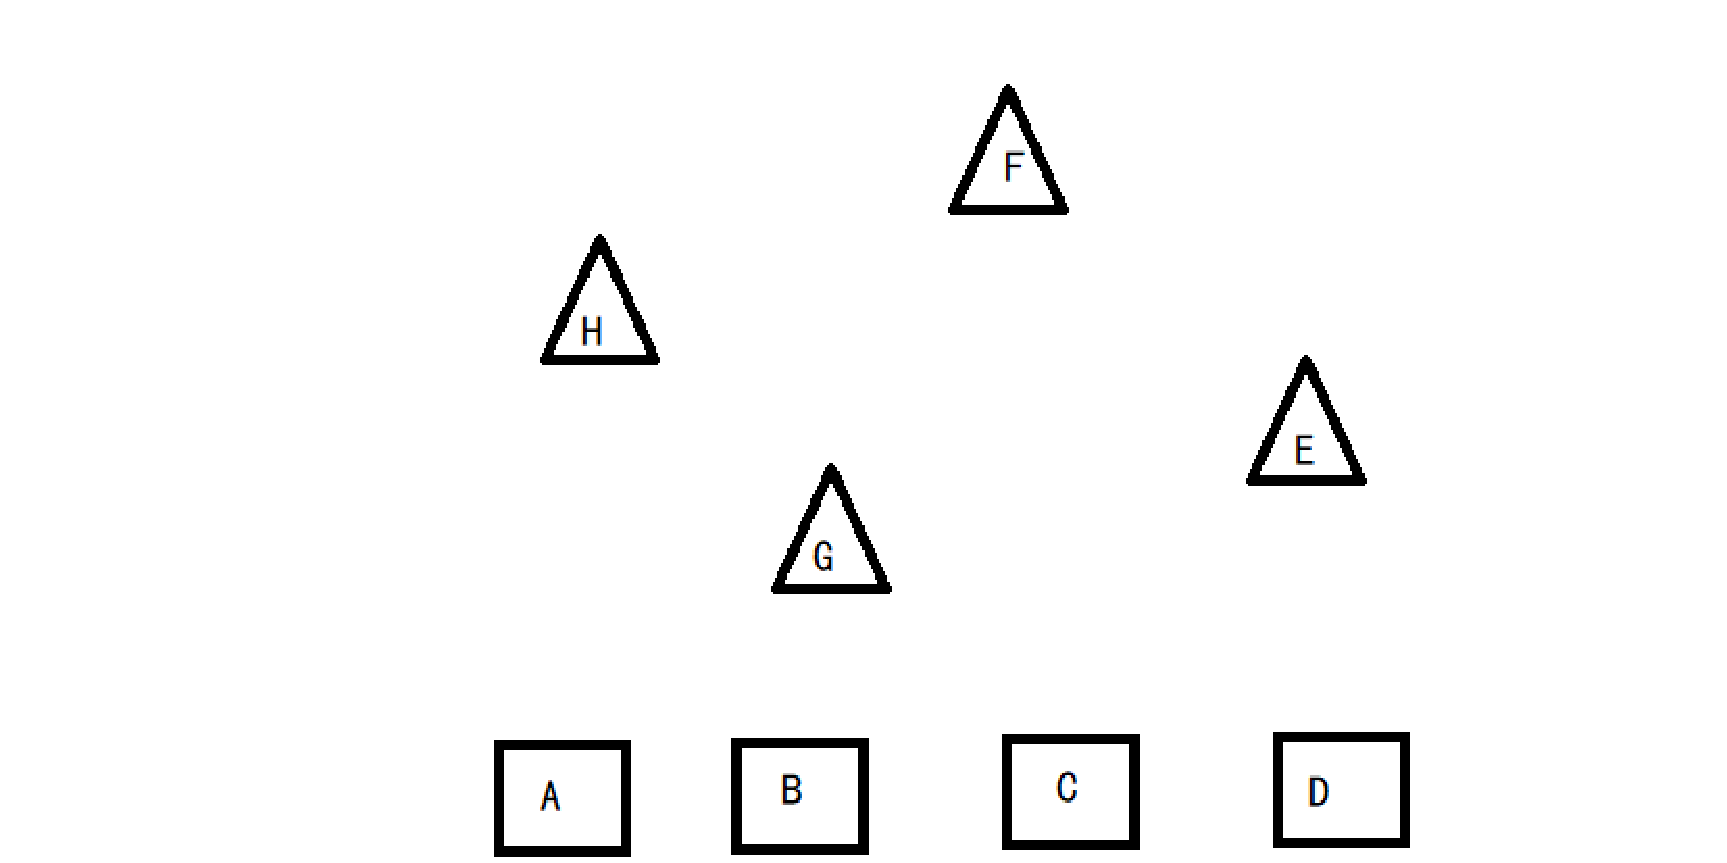
\includegraphics[width=0.6\linewidth]{g1.pdf}
\caption{两类分类问题中8个样本的分布图}
\label{fig:g1}
\end{figure}

%%%%%%%%%%%%%%%%%%%%%%%%%%%%%%%%%%%%%%%%%%%%%%%%%%%%%%%%%%%%%%%%%%%%%%%%%
% Problem 2
%%%%%%%%%%%%%%%%%%%%%%%%%%%%%%%%%%%%%%%%%%%%%%%%%%%%%%%%%%%%%%%%%%%%%%%%%%%%%%%%%%%%%%%%%%%%%%%%%%%%%%%%%%%%%%%%%%%%%%%%%%%%%%%%%%%%%%%%

\begin{problem}{2}
加入L2标准化(normalization)后，线性回归的损失函数的标准形式为:
 $$L=(Y-X w)^T(Y-X w)+ \lambda w^t w,\qquad \lambda > 0$$
\begin{enumerate}[1)]
    \item 假设L2标准化项被误写为$\lambda Y^ TY$，请解释为什么该项起不到标准化的作用。
    \item 假设L2标准化正确，但$\lambda$小于0，请解释为什么该项起不到标准化的作用。
\end{enumerate}
\end{problem}

%%%%%%%%%%%%%%%%%%%%%%%%%%%%%%%%%%%%%%%%%%%%%%%%%%%%%%%%%%%%%%%%%%%%%%%%%
% Problem 3
%%%%%%%%%%%%%%%%%%%%%%%%%%%%%%%%%%%%%%%%%%%%%%%%%%%%%%%%%%%%%%%%%%%%%%%%%%%%%%%%%%%%%%%%%%%%%%%%%%%%%%%%%%%%%%%%%%%%%%%%%%%%%%%%%%%%%%%%

\begin{problem}{3}
考虑下面如表1所示的一个数据集，它记录了某学生多次考试的情况，请根据提供的数据按要求构建决策树。
\begin{enumerate}[1)]
    \item 根据信息增益率选择第一个属性，构建一个深度为1的决策树（根节点的深度为 1）。
    \item 根据信息增益率构建完整的决策树。请回答，这两个决策树的决策结果是否和训练数据一致，并解释说明。
\end{enumerate}
\end{problem}

\begin{table}[h]
    \centering
    \caption{某学生多次考试情况}
    \label{tab:number}
    \begin{tabular}{ccc}
        \hline
        是否通过考试 & 是否认真复习 & 是否超常发挥 \\
        \hline \hline
        是 & 是 & 否 \\ \hline
        是 & 是 & 是 \\ \hline
        是 & 是 & 否 \\ \hline
        是 & 是 & 是 \\ \hline
        是 & 是 & 否 \\ \hline
        是 & 否 & 是 \\ \hline
        否 & 否 & 否 \\ \hline
        否 & 否 & 是 \\ \hline
    \end{tabular}
\end{table}

%%%%%%%%%%%%%%%%%%%%%%%%%%%%%%%%%%%%%%%%%%%%%%%%%%%%%%%%%%%%%%%%%%%%%%%%%
% Problem 4
%%%%%%%%%%%%%%%%%%%%%%%%%%%%%%%%%%%%%%%%%%%%%%%%%%%%%%%%%%%%%%%%%%%%%%%%%%%%%%%%%%%%%%%%%%%%%%%%%%%%%%%%%%%%%%%%%%%%%%%%%%%%%%%%%%%%%%%%

\begin{problem}{4}
考虑如表2所示的一个数据集，对于如下数据，考虑使用Ada boosting方法来训练"是否出去玩"强分类器。每个弱分类器可考虑对单个属性的分类，比如对于“心情指数”这一属性，可考虑心情指数 $>2$和心情指数$<4$两个方面。请回答下列问题。
\begin{enumerate}[1)]
    \item Ada boosting在第一轮迭代中将会选择哪一个弱分类器？
    \item 第一轮迭代前与迭代后每个样本的权重是多少？
    \item 第二轮迭代选择的弱分类器是哪一个？分类器的权重是多少。
    \item 写出三轮迭代后的强分类器的表达式（每个弱分类器可用字母替代）。
\end{enumerate}
\end{problem}

\begin{table}[h]
    \centering
    \caption{是否出去玩决策数据}
    \label{tab:number}
    \begin{tabular}{ccccccc}
        \hline
        序号 & 出去玩 & 天气状况 & 有同伴 & 零花钱 & 特殊节日 & 心情指数(1差5好) \\
        \hline \hline
        1 & 是 & 好 & 无 & 多 & 是 & 5 \\ \hline
        2 & 是 & 一般 & 有 & 多 & 是 & 5 \\ \hline
        3 & 是 & 一般 & 有 & 少 & 否 & 1 \\ \hline
        4 & 是 & 一般 & 有 & 少 & 否 & 3 \\ \hline
        5 & 是 & 一般 & 有 & 少 & 否 & 5 \\ \hline
        6 & 是 & 好 & 无 & 多 & 是 & 5 \\ \hline
        7 & 是 & 好 & 无 & 多 & 是 & 5 \\ \hline
        8 & 否 & 一般 & 无 & 多 & 是 & 1 \\ \hline
        9 & 否 & 一般 & 有 & 少 & 否 & 1 \\ \hline
        10 & 否 & 一般 & 无 & 少 & 否 & 5 \\ \hline
    \end{tabular}
\end{table}

\newpage
\noindent\rule{7in}{1pt}
\textbf{第二部分：实训题（共4分）}
\\ \\
\textbf{实训题要求:}
\begin{itemize}
    \item 本次作业包括1个实训题，作业要求以及基础代码以Aistudio项目的形式发布。
    \item 发布项目链接有效期3天，请在作业发布3天内fork这个项目，生成``我的项目''，并在自己fork的项目下进行作答，生成答案后按要求保存提交。
\end{itemize}

%%%%%%%%%%%%%%%%%%%%%%%%%%%%%%%%%%%%%%%%%%%%%%%%%%%%%%%%%%%%%%%%%%%%%%%%%
% Problem 1
%%%%%%%%%%%%%%%%%%%%%%%%%%%%%%%%%%%%%%%%%%%%%%%%%%%%%%%%%%%%%%%%%%%%%%%%%%%%%%%%%%%%%%%%%%%%%%%%%%%%%%%%%%%%%%%%%%%%%%%%%%%%%%%%%%%%%%%%

\begin{problem}{1 二分类-垃圾短信分类识别}

    垃圾短信 (Spam Messages，SM) 是指未经过用户同意向用户发送不愿接收的商业广告或者不符合法律规范的短信。
随着手机的普及，垃圾短信在日常生活日益泛滥，已经严重的影响到了人们的正常生活娱乐，乃至社会的稳定。

本实验要求使用Pandas, Numpy, Sklearn 等库进行相关特征处理，使用 Sklearn 框架训练分类器，使用机器学习的方法对垃圾短信进行分类。

实验介绍详情和参考基础代码请参见Aistudio中的共享项目\href{https://aistudio.baidu.com/studio/project/partial/verify/7582660/d72871e3eb6146cfb4d9fdafa4ca3116}{“人工智能课程-作业一-垃圾短信分类”}。

\end{problem}

\noindent\rule{7in}{1pt}
\textbf{第三部分：实训题实验报告（共2分）}
\begin{itemize}
    \item 请按照实验报告模板完成实验报告。
    \item 实验报告模板是通用模板，可根据每个作业要求的差别，自由进行微调。
\end{itemize}

\end{CJK}
\end{document}